% Appendix A

\chapter{Example Plots} % Main appendix title

\label{AppendixB} % For referencing this appendix elsewhere, use \ref{AppendixA}

\lhead{Appendix B. \emph{Example Plots}} % This is for the header on each page - perhaps a shortened title

\begin{figure}[H]
  \centering
    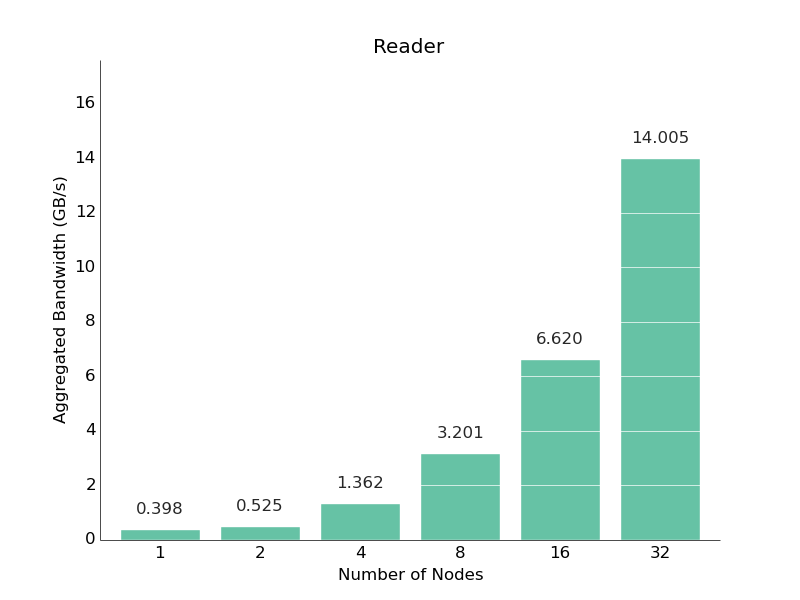
\includegraphics[scale=0.6]{Figures/amfora_32_n_to_1.png}
    \rule{25em}{0.5pt}
  \caption[AMFS, N-to-1 read]{AMFS, N-to-1 read}
  \label{fig:plot1}
\end{figure}

\begin{figure}[H]
  \centering
    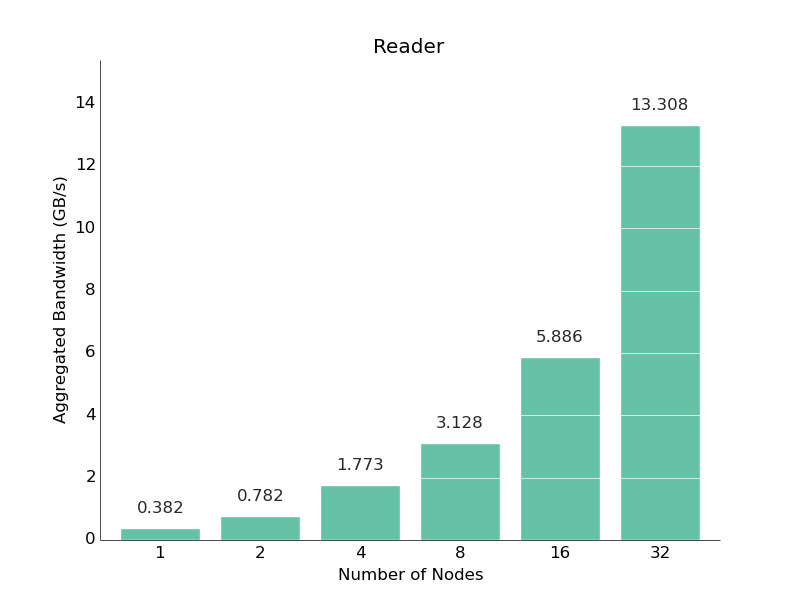
\includegraphics[scale=0.6]{Figures/amfora_32_1_to_1.png}
    \rule{25em}{0.5pt}
  \caption[AMFS, 1-to-1 read]{AMFS, 1-to-1 read}
  \label{fig:plot2}
\end{figure}

\begin{figure}[H]
  \centering
    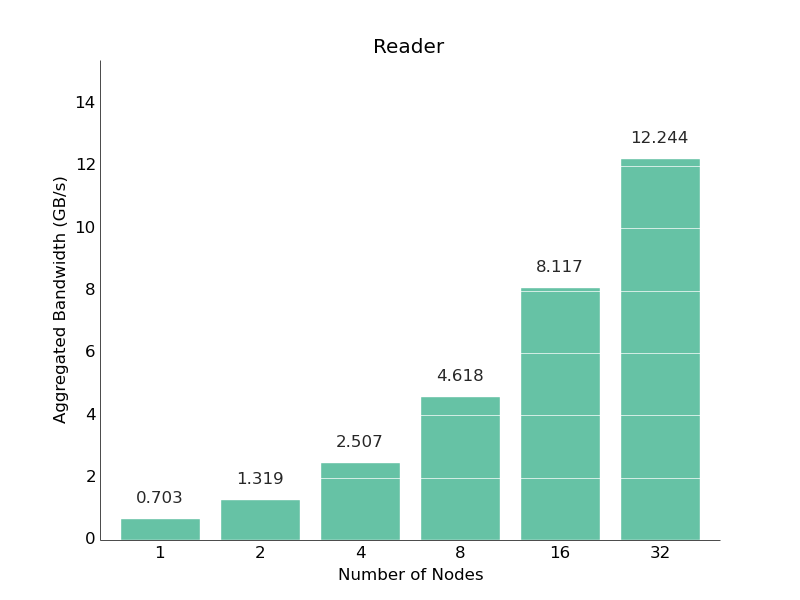
\includegraphics[scale=0.6]{Figures/memfs_32_1_to_1.png}
    \rule{25em}{0.5pt}
  \caption[AMFS, N-to-1 read]{MemFS, N-to-1 read}
  \label{fig:plot3}
\end{figure}

\begin{figure}[H]
  \centering
    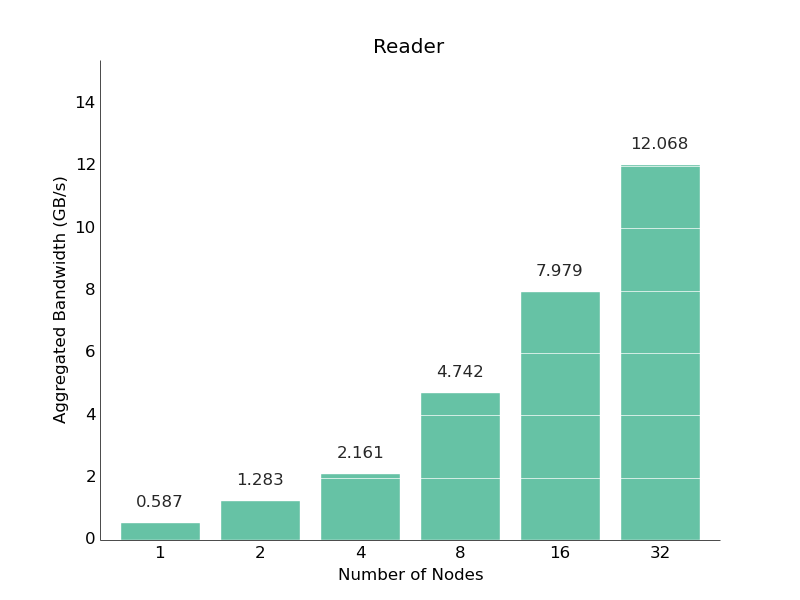
\includegraphics[scale=0.6]{Figures/memfs_32_N_to_1.png}
    \rule{25em}{0.5pt}
  \caption[AMFS, N-to-1 read]{MemFS, 1-to-1 read}
  \label{fig:plot4}
\end{figure}

% TODO - mdtest plots